\section*{\MakeUppercase{Preface}}
\addcontentsline{toc}{section}{\MakeUppercase{Preface}}

%%
%%   If your work (dissertation/thesis) has a Preface,
%%   place its text below instead of lines 9-26
%% 

Hello, world! This is an example of a dissertation formatted according to the guidelines of \ac{umkc}.\footnote{An example of footnote.} Below is an example of image placed in Figure~\ref{fig:image1}, p.~\pageref{fig:image1}.

\begin{figure}[!ht]
    \vspace{.4in}
    % The figure's caption and notes lines are centered, 75% of page width 
    \captionsetup{width=.75\linewidth,labelfont=bf}
    \caption{Example of an image sized to 75\% of the page width}
    \vspace{.2in}
    \centering
    % The plot is 75% of its width
    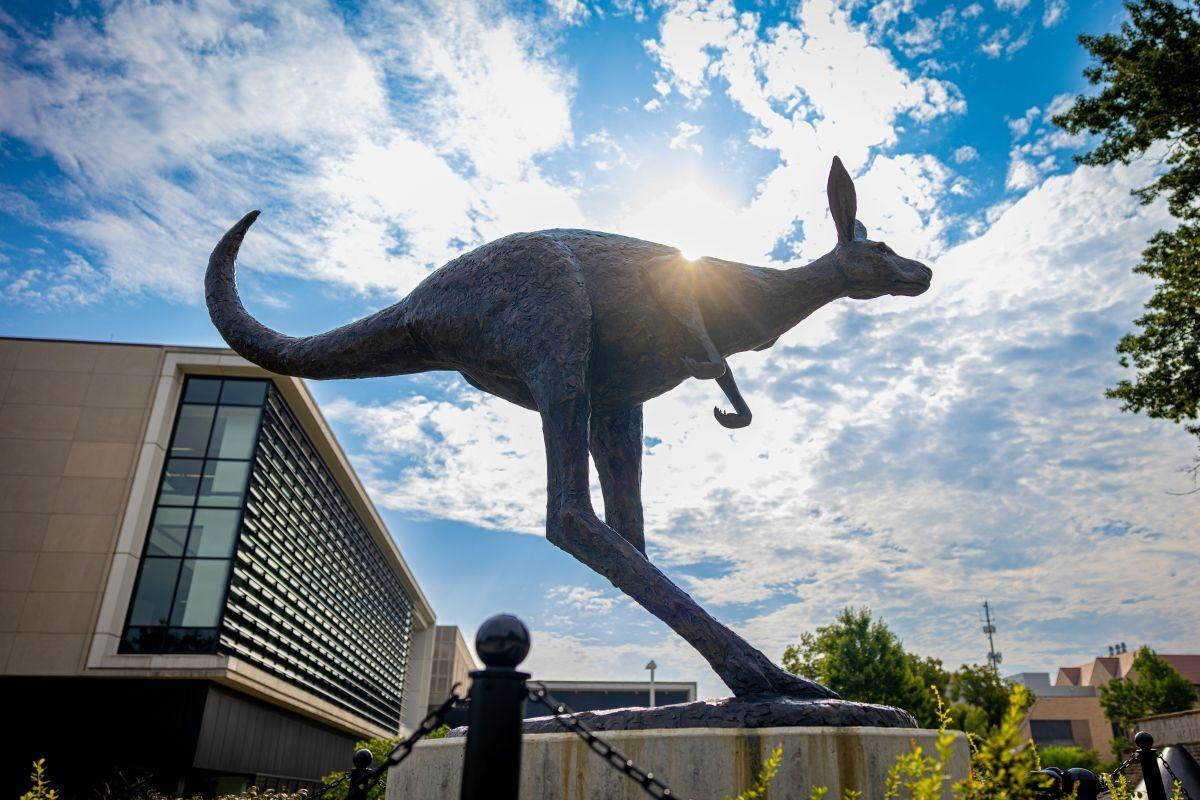
\includegraphics[width=.75\linewidth]{Images/UMKC_Roos.jpg}
    \vspace{.2in}
    \caption*{Note: some notes. \par\vspace{.15in} Source: \ac{umkc}, \url{https://www.umkc.edu/}}
    \vspace{.2in}
    \label{fig:image1}
\end{figure}

\lipsum[1-3] % text fill, random text